\documentclass[a4paper,twoside,12pt]{article}
%\usepackage [reqno] {amsmath}


% //////////////////// Pakete laden ////////////////////
\usepackage{amsmath}			% MUSS vor fontspec geladen werden
\usepackage{mathtools}			% modifiziert amsmath
\usepackage{amssymb}			% mathematische symbole, für \ceckmarks
\usepackage{amsthm}				% für proof
\usepackage{mathrsfs}			% für \mathscr
\usepackage{latexsym}
\usepackage{marvosym}				% für Lightning

\usepackage{fontspec} 			% funktioniert nur mit den neueren Compilern z.B. XeLaTeX
\usepackage{microtype}			% für bessere Worttrennung
\usepackage[ngerman]{babel} 	% Spracheinstellung
\usepackage{lmodern}			% verändert verwendete Schriftart, damit sie weniger pixelig ist

\usepackage{verbatim}
\usepackage{listings}			% Für Quellcode

\usepackage{graphicx}
%\usepackage{subcaption}
\usepackage{subfig}
\usepackage{tabularx}			% für Tabellen mit gleicher Spaltenbreite und automatischen Umbrüchen
\usepackage{fullpage}
\usepackage{multirow}			% für multirow in tabulars
\usepackage{rotate}
\usepackage[cmyk,table]{xcolor} % um Farben zu benutzen, kann mehr als das Paket color
\usepackage[					% Verlinkungen
	colorlinks,					% farbige Schrift, statt farbiger Rahmen
	linktocpage,				% verlinkt im Abb.Verzeichnis Seitenzahl statt Bildunterschrift
	linkcolor=blue				% setzt Farbe der Links auf blau
	]{hyperref}					% nur für digitale Anwendungen, url = "http://www.example.com"
\usepackage{url}				% für Webadressen wie e-mail usw.: "\url{http://www.example.com}"

\usepackage{enumerate}			% für versch. Aufzählungezeichen wie z.B. a)
\usepackage{xspace}				% folgt ein Leerzeichen nach einem \Befehl, wird es nicht verschluckt.
\usepackage{cancel}				% für das Durchstreichen u.a. in Matheformeln mit \cancel
\usepackage{float}              % zum Forcieren der Position von figure-Umgebungen

% zum Zeichnen (u.a. von Graphen)
\usepackage{fp}
\usepackage{tikz}
\usetikzlibrary{tikzmark}			% für \tikzmark{toRemember}
\usetikzlibrary{positioning}	% verbesserte Positionierung der Knoten
\usetikzlibrary{automata}		% für Automaten (GTI)
\usetikzlibrary{arrows}
\usetikzlibrary{shapes}
\usetikzlibrary{decorations.pathmorphing}
\usetikzlibrary{decorations.pathreplacing}
\usetikzlibrary{decorations.shapes}
\usetikzlibrary{decorations.text}

% //////////////////// Syntaxhighlighting ////////////////////
\lstloadlanguages{Python, Haskell, [LaTeX]TeX, Java}
\lstset{
   basicstyle=\footnotesize\ttfamily,	% \scriptsize the size of the fonts that are used for the code
   backgroundcolor = \color{bgcolour},	% legt Farbe der Box fest
   breakatwhitespace=false,	% sets if automatic breaks should only happen at whitespace
   breaklines=true,			% sets automatic line breaking
   captionpos=t,				% sets the caption-position to bottom, t for top
   commentstyle=\color{codeblue}\ttfamily,% comment style
   frame=single,				% adds a frame around the code
   keepspaces=true,			% keeps spaces in text, useful for keeping indentation
							% of code (possibly needs columns=flexible)
   keywordstyle=\bfseries\ttfamily\color{codepurple},% keyword style
   numbers=left,				% where to put the line-numbers;
   							% possible values are (none, left, right)
   numberstyle=\tiny\color{codegreen},	% the style that is used for the line-numbers
   numbersep=5pt,			% how far the line-numbers are from the code
   stepnumber=1,				% nummeriert nur jede i-te Zeile
   showspaces=false,			% show spaces everywhere adding particular underscores;
							% it overrides 'showstringspaces'
   showstringspaces=false,	% underline spaces within strings only
   showtabs=false,			% show tabs within strings adding particular underscores
   flexiblecolumns=false,
   tabsize=1,				% the step between two line-numbers. If 1: each line will be numbered
   stringstyle=\color{orange}\ttfamily,	% string literal style
   numberblanklines=false,				% leere Zeilen werden nicht mitnummeriert
   xleftmargin=1.2em,					% Abstand zum linken Layoutrand
   xrightmargin=0.4em,					% Abstand zum rechten Layoutrand
   aboveskip=2ex, 
}

\lstdefinestyle{py}{
   language=Python,
}
\lstdefinestyle{hs}{
   language=Haskell,
}
\lstdefinestyle{html}{
   language=HTML,
}
\lstdefinestyle{tex}{
	language=[LaTeX]TeX,
	escapeinside={\%*}{*)},     % if you want to add LaTeX within your code
	texcsstyle=*\bfseries\color{blue},% hervorhebung der tex-Schlüsselwörter
	morekeywords={*,$,\{,\},\[,\],lstinputlisting,includegraphics,
	rowcolor,columncolor,listoffigures,lstlistoflistings,
	subsection,subsubsection,textcolor,tableofcontents,colorbox,
	fcolorbox,definecolor,cellcolor,url,linktocpage,subtitle,
	subject,maketitle,usetikzlibrary,node,path,addbibresource,
	printbibliography},% if you want to add more keywords to the set
     numbers=none,
     numbersep=0pt,
     xleftmargin=0.4em,
}

\lstdefinestyle{java}{
	language=Java,
	extendedchars=true,		% lets you use non-ASCII characters;
   						% for 8-bits encodings only, does not work with UTF-8
}

\lstdefinelanguage[x64]{Assembler}     % add a "x64" dialect of Assembler
   [x86masm]{Assembler} % based on the "x86masm" dialect
   % with these extra keywords:
   {morekeywords={CDQE,CQO,CMPSQ,CMPXCHG16B,JRCXZ,LODSQ,MOVSXD, %
                  POPFQ,PUSHFQ,SCASQ,STOSQ,IRETQ,RDTSCP,SWAPGS, %
                  rax,rdx,rcx,rbx,rsi,rdi,rsp,rbp, %
                  r8,r8d,r8w,r8b,r9,r9d,r9w,r9b}
}					% for 8-bits encodings only, does not work with UTF-8

\lstdefinestyle{c}{
	language=c,
	extendedchars=true,		% for 8-bits encodings only, does not work with UTF-8
}

\newcommand{\ZETTELNUMMER}{2}

\newcounter{AUFGNR}
\setcounter{AUFGNR}{1}
\newcommand{\AUFGABE}[2]{\vspace{0.3cm}\item[Aufgabe~\arabic{AUFGNR}]\stepcounter{AUFGNR} #1\hfill\emph{#2}}


\newcommand{\floor}[1]{\left\lfloor{#1}\right\rfloor}
\newcommand{\ceil}[1]{\left\lceil{#1}\right\rceil}
\newcommand{\half}[1]{\frac{#1}{2}}
\newcommand{\N}{\mathbb{N}}



\renewcommand{\labelenumi}{(\alph{enumi})}
\renewcommand{\labelenumii}{(\roman{enumii})}

% //////////////////// eigene Farben ////////////////////
\let\definecolor=\xdefinecolor
\definecolor{FUgreen}{RGB}{153,204,0}
\definecolor{FUblue}{RGB}{0,51,102}

\definecolor{middlegray}{rgb}{0.5,0.5,0.5}
\definecolor{lightgray}{rgb}{0.8,0.8,0.8}
\definecolor{orange}{rgb}{0.8,0.3,0.3}
\definecolor{azur}{rgb}{0,0.7,1}
\definecolor{yac}{rgb}{0.6,0.6,0.1}
\definecolor{Pink}{rgb}{1,0,0.6}

\definecolor{bgcolour}{rgb}{0.97,0.97,0.97}
\definecolor{codegreen}{rgb}{0,0.6,0}
\definecolor{codegray}{rgb}{0.35,0.35,0.35}
\definecolor{codepurple}{rgb}{0.58,0,0.82}
\definecolor{codeblue}{rgb}{0.4,0.5,1}


\begin{document}
\pagestyle{empty}
\hrule\medskip
\rule{0ex}{0ex}\\[-1ex]
\ZETTELNUMMER. Aufgabenblatt zur Vorlesung

\smallskip
\noindent
\large
\textbf{Nichtsequentielle und Verteilte Programmierung}\hfill SoSe
2018 \\[0.5ex]
Tutorium No. 04 bei Johannes Nixdorf\\[0.5ex]

\normalsize
Anton Oehler, Mark Niehues

\medskip\hrule

\begin{description}
\AUFGABE{Nebenläufiges Zählen}{}
\begin{enumerate}
\item Durch das cachen der Variablen n, kann diese beliebige Werte zwischen \textit{K} und \textit{-K} am Ende des Programmablaufes annehmen. Bei Annahme schwacher Fairness ist davon auszugehen, dass einer der Threads zu einem Zeitpunkt, da \texttt{n} nicht mehr null ist, seiner eigenen Cache Variablen diesen Wert zuweist. Was zwischen dem Cachen und dem zurückschreiben im nächsten atomaren Schritt eines Threads passiert, hat keine Auswirkungen auf den End-Zustand des Programms. Dementsprechend hängt der End-Zustand nur davon ab, an welcher stelle die Variable \texttt{n} gecached bzw. in diesem Fall könnte man auch sagen \textit{eingefroren} wird.

\item \lstinputlisting[style=java,								% Style
	firstnumber={1},										% Start der Nummerierung
	firstline={0}											% 1. Codezeile
]											% letzte Codezeile
{./Aufgabe1.java}

\end{enumerate}

\AUFGABE{Parallele Suche}{}

Es lässt sich zeigen, dass Programm \textit{a} und \textit{b} aus den selben Gründen nicht korrekt sind, während Programm \textit{c} korrekt ist. Die Ursache für das Fehlerhafte verhalten der ersten beiden Programme bildet der Umstand, dass die \texttt{found} Variable auch mit \texttt{false} überschrieben wird, falls ein Thread keine Nullstelle gefunden hat. Dadurch kann das Finden der Nullstelle bei ungünstigem Schedulen untergehen. Mit diesem Fall ist auf Grund der angenommenen schwachen Fairness zu rechnen. Ein Szenario zu Programm \textit{a} wäre besipielsweise (das Szenario zu \textit{b} ist analog):
\lstinputlisting[
	caption={Beispielhaftes Szenario, dass die Korrektheit von a widerlegt.},								% Style
	firstnumber={1},										% Start der Nummerierung
	firstline={0}											% 1. Codezeile
]											% letzte Codezeile
{./Aufgabe2.txt}

In dem letzten Programm kann die Variable, die anzeigt, dass eine Nullstelle gefunden wurde nicht mehr mit \texttt{false} überschrieben werden sobald sie einmal den Wert \texttt{true} zugewiesen bekommen hat. Dadurch terminieren beide Threads zwangsläufig, sobald einer der beiden die Nullstelle gefunden hat.

\AUFGABE{Das Froschpuzzle}{}
\begin{figure}[htbp] 
  \centering
     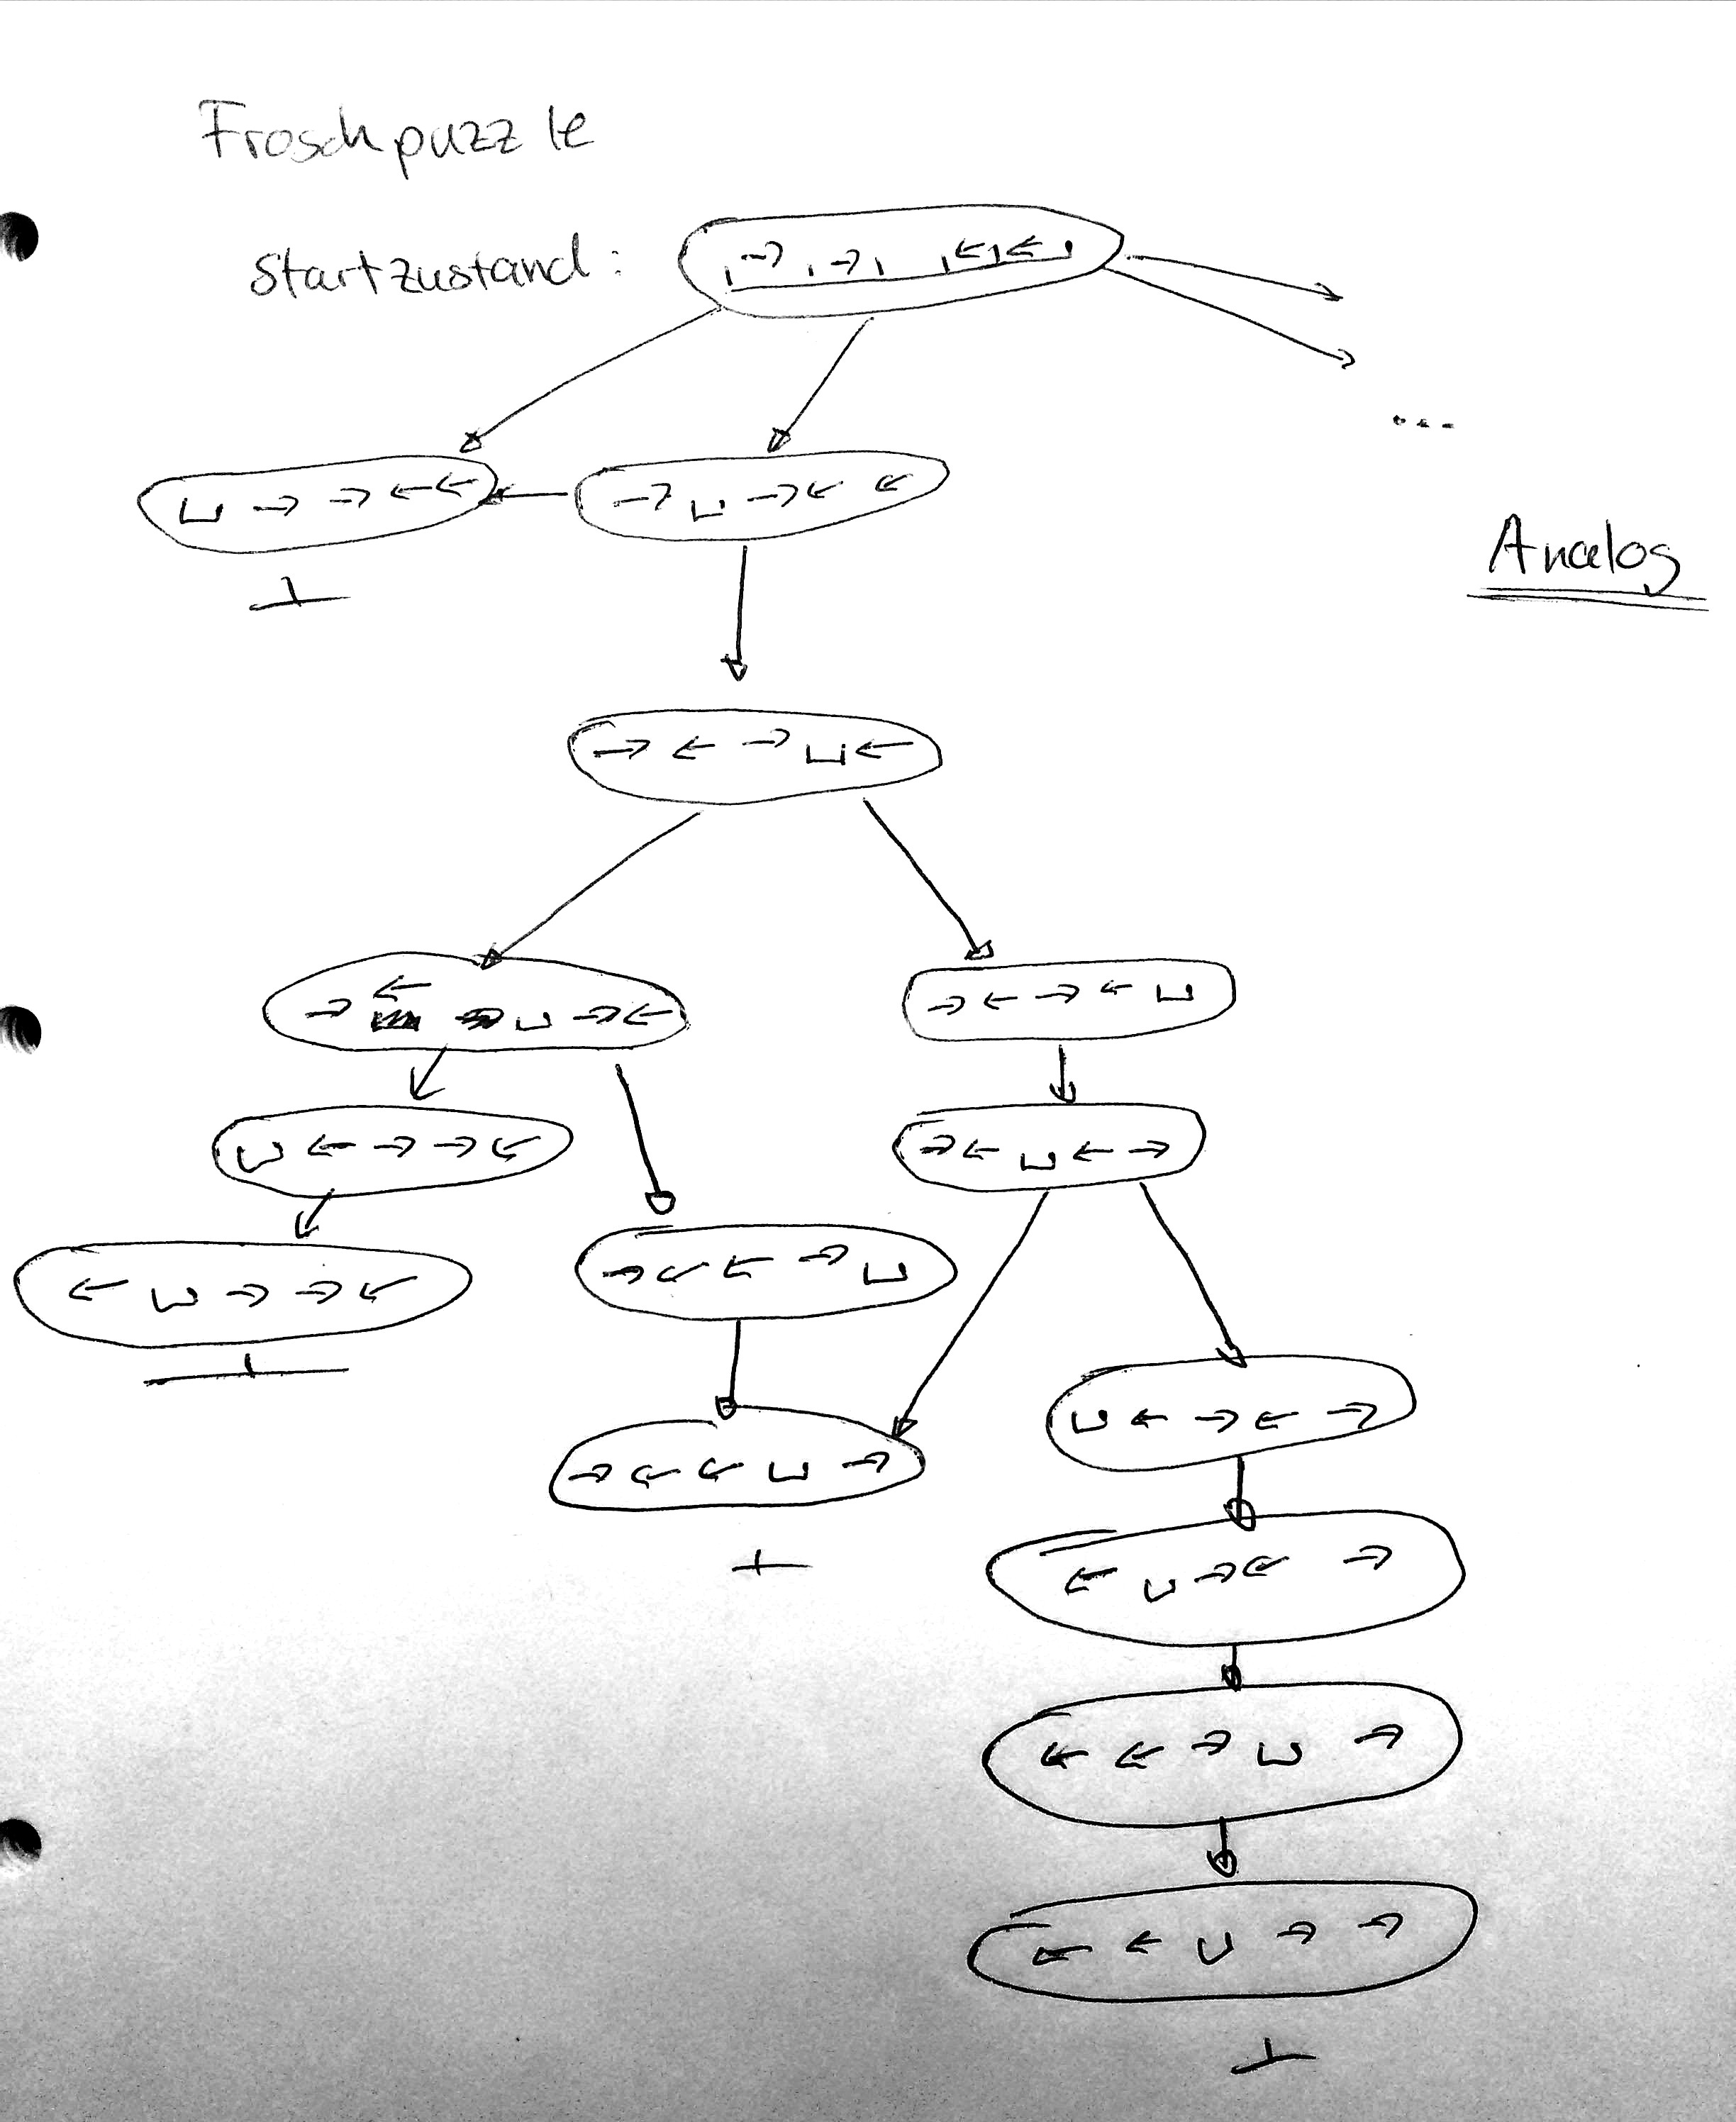
\includegraphics[width=0.8\textwidth]{frog.jpg}
  \caption{Zustandsdiagramm des Froschpuzzles}
\end{figure}
\end{description}
\end{document}